\newpage
\section{Informații preliminarii}
Topologia, ca și o ramură bine definită a matematicii, își are originiile de la începutul secolului XX, 
însa au fost descoperite și cazuri izolate în aplicarea acestui concept chiar și cu câteva secole în urmă. 
Leonhard Euler este considerat ca fiind primul care abordează acest domeniu prin lucrarea sa scrisa în 1736, 
Cele șapte poduri din Konigsberg, care se referă la crearea unui traseu prin orașul Konigsberg trecând peste fiecare pod o 
singură dată, lucru ce sa dovedit imposibil. (figura 1) \newline

\begin{figure}[H]
    \begin{center}
        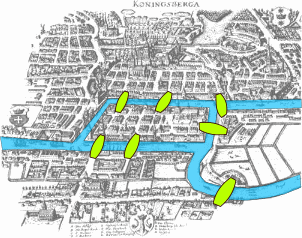
\includegraphics[scale=0.60]{imagini/istorie/bridge.png}        
    \end{center}    
        \caption{Cele șapte poduri din Konigsberg  \protect\footnotemark}
                    
    \label{fig:poduri}
\end{figure}

\footnotetext{\url{https://en.wikipedia.org/wiki/Topology/media/File:Konigsberg\_bridges.png}}

La 14 noiembrie 1750, Euler a scris unui prieten că a realizat importanța muchiilor unui poliedru. 
Aceasta a condus la formula lui poliedrala \cite{topolgy}: \[V-E+F=2\] unde \(V\), \(E\) și \(F\) indică numărul de vârfuri, 
muchii și fețe ale poliedrului. Această analiză este considerată drept prima teoremă, semnalizând nașterea 
topologiei.\newline

Alte contribuții au fost făcute de Augustin-Louis Cauchy, Ludwig Schläfli, Johann Benedict Listing, 
Bernhard Riemann și Enrico Betti. Listing a introdus termenul "Topologie" în "Vorstudien zur Topologie", 
scris în limba germană.\newline 
